\chapter{What is Calculus?}
\label{ch:whatiscalculus}

\begin{center}
``The calculus was the first achievement of modern mathematics and it is difficult to overestimate its importance." (John von Neumann)
\end{center}

%\addcontentsline{toc}{chapter}{What is Calculus?}
\begin{wrapfigure}{R}{0.25\textwidth}
  %\vspace{-20pt}
  \centering
    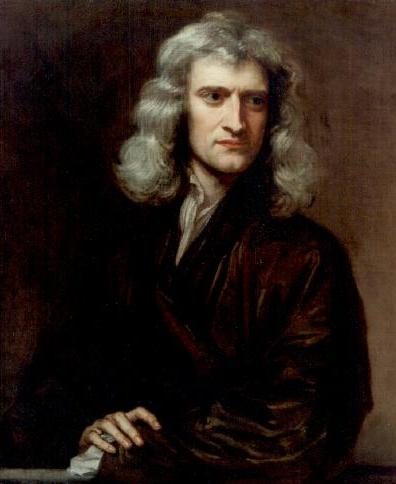
\includegraphics[width=0.24\textwidth]{img/chap0/IsaacNewton.jpg}
  %\end{center}
%\vspace{-20pt}  
\caption{Isaac Newton in 1689}
%\vspace{-10pt}
\end{wrapfigure}

A good speaker will often begin a talk with an outline of what will be discussed in the talk. In the same way, it is incumbent upon the author of a textbook to give the reader the big picture of the subject of the textbook. That is the purpose of this brief chapter.

\paragraph{Calculus is the study of change.} Over time, the population of a city may grow. The price of a stock will fluctuate: sometimes increasing and sometimes decreasing. The cumulative profits of a company may grow or wane. These situations represent changing quantities. We may want to dig deeper and find out how quickly the city is growing or the rate at which a company's stock price or profits are growing. Those are questions that calculus attempts to answer.

\begin{wrapfigure}{R}{0.25\textwidth}
%\vspace{-20pt} 
 \centering
    \includegraphics[width=0.24\textwidth]{img/chap0/GottfriedWilhelmLeibniz.jpg}
  %\end{center}
%\vspace{-20pt}
  \caption{Gottfried Wilhelm Leibniz circa 1695}
%\vspace{-10pt}
\end{wrapfigure}

Calculus was first developed in the late 1600s independently by Sir Isaac Newton\index{Newton, Isaac} and Gottfried Wilhelm Leibniz\index{Leibniz, Gottfried} to help them describe and understand the rules governing the motion of planets and moons. Since then, thousands of other men and women have refined the basic ideas of calculus, developed new techniques to make the calculations easier, and found ways to apply calculus to problems besides planetary motion. Perhaps most importantly, they have used calculus to help understand a wide variety of physical, biological, economic, and social phenomena and to describe and solve problems in those areas.


Part of the beauty of calculus is that it is based on a few very simple ideas. Part of the power of calculus is that these simple ideas can help us understand, describe, and solve problems in a variety of fields.

\section{Two Problems}
\label{sec:twoproblems}

Calculus is the study of two seemingly different questions that are actually inverses of each other.
\begin{enumerate}
    \item What is the {\bf rate of change}\index{Rate of change} of a function?
    \item What is the {\bf accumulation}\index{Accumulation} of a function?
\end{enumerate}
Geometrically, these questions can be visualized as the {\bf slope of a curve}\index{Slope!curve} and the {\bf area under a curve}\index{Area!under a curve}, respectively, as seen in Figure \ref{fig:0-1}. We start with these pictures because a conceptual understanding of calculus (and really, all of mathematics), and not merely as a set of rules and procedures, is crucial to understanding the content of this course and being able to apply it to real-world problems, perhaps even in novel ways.

\begin{figure}[h!]
    \centering
    \begin{subfigure}[b]{0.45\textwidth}
        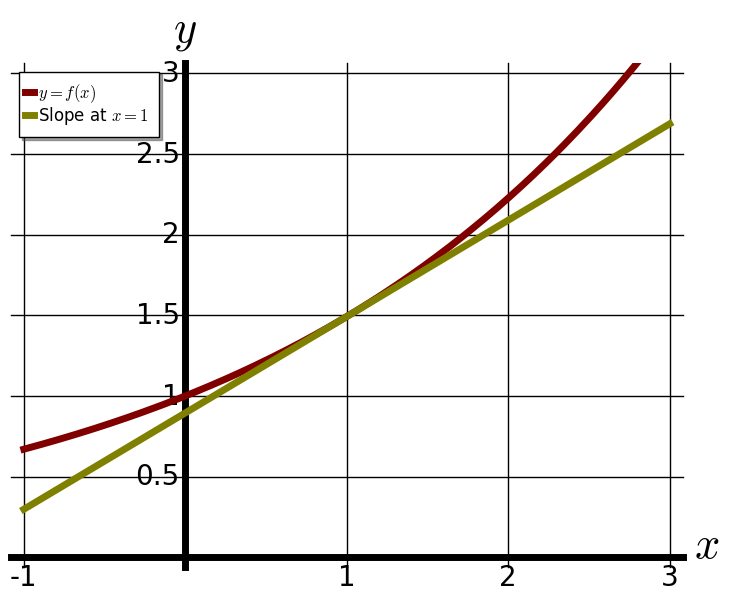
\includegraphics[width=\textwidth]{img/chap0/ex0-1.png}
        \caption{Slope of a Curve at a Point}
        \label{fig:0slope}
    \end{subfigure}
    ~ %add desired spacing between images, e. g. ~, \quad, \qquad, \hfill etc.
    \begin{subfigure}[b]{0.45\textwidth}
        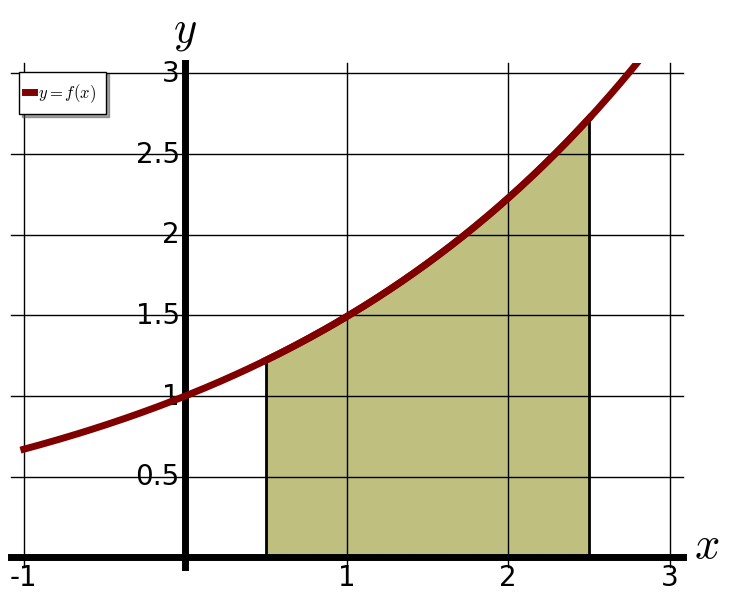
\includegraphics[width=\textwidth]{img/chap0/ex0-2.png}
        \caption{Area Under a Curve over an Interval}
        \label{fig:0area}
    \end{subfigure}
    \caption{Visualizing the Two Problems of Calculus}\label{fig:0-1}
\end{figure}

In this book, we will unpack these two problems and two pictures and show how they are useful to business, economics, finance, the social sciences, and the life sciences. We will take a data-driven and a problem-solving approach to this course, working with real and realistic data. Yes, all of calculus is derived from understanding those two pictures. Study those two pictures again.

Let's consider a pair of examples to illustrate these two concepts.

\begin{example}
Suppose that you're paid $y$ dollars for working $x$ hours. A graph of the relationship between the amount of time you work (in hours) and your pay (in dollars) is in Figure \ref{fig:0-rate}. The slope of the line is your hourly pay rate. In this case, the slope of the curve and the rate of change of the function is \$15 per hour.
\begin{figure}[h!]
\centering
\begin{tikzpicture}[scale=0.1]
    % grid
    \draw[step=10, very thin, gray] (0, 0) grid (40, 60);

    % axes
    \draw[->] (-2,0) -- coordinate (x axis mid) (42,0) node[right] {$x$};
    \draw[->] (0,-2) -- coordinate (y axis mid) (0,63) node[above] {$y$};

    % ticks
    \foreach \x in {10, 20, ..., 40}
     		\draw (\x,1pt) -- (\x,-3pt)
			node[anchor=north] {\x};
    	\foreach \y in {100, 200, ..., 600}
     		\draw (1pt,\y/10) -- (-3pt,\y/10) 
     			node[anchor=east] {\y}; 

    % labels
    \node[below = 15] at (x axis mid) {Hours worked};
	\node[rotate=90, above = 25] at (y axis mid) {Pay (U.S.\ Dollars)};

    % plot 
    \draw[->, thick, color=aldRed] (0, 0) -- (42, 63);
    
    % legend

\end{tikzpicture}
\caption{Pay as a function of time worked.}
\label{fig:0-rate}
\end{figure}
\end{example}

\begin{example}
Suppose that $t$ hours after a snowstorm starts, the snowfall rate is $r(t)$ inches per hour. The shaded area represents the total accumulation of the snow during the storm.
\end{example}

\section{Problem Solving}
\label{sec:polya}

One day when my wife was pregnant with our second child, she was lying down on the couch with a bit of nausea, which is not uncommon in the first trimester. I offered her a ginger candy, which helps to alleviate nausea. Our son, who was a clever two years old at the time asked me, ``Pwease I have ginger candy?" I replied, ``No, you can't have ginger candy. It's for mommy. Mommy's tummy hurts." My son sat for a minute thinking. After a moment, he said. ``My tummy hurts. Pwease I have ginger candy?" He still didn't get the candy; we don't reward dishonesty, but it was a humorous example of problem solving.

Have you ever looked at a math problem and said to yourself, ``I don't know where to start!" No matter how you answered that question, this section will offer some tips.

One often thinks of the study of a mathematical subject as mere rote memorization of formulas and step-by-step procedures. On the contrary, the approach that mathematicians take to the subject is much more creative. We see mathematics as a way to apply abstract concepts to solve problems. Often there is just one correct answer. Often, however, the ``correct" or ``best" answer may be impossible to find, so we are instead interested in a solution that would be considered ``good," ``plausible," or ``reasonable." That is the approach that will drive much of the content of this textbook. In short, one of our objectives is to retrain the way you view mathematics: it's not about knowing or not knowing the answer, it's about figuring out a solution. This textbook is not a book to tell you what to think, but how to think about quantitative problem solving.

In light of this, we introduce a well-known problem-solving process and thoughts on how to implement it in practice. In his famous book {\em How to Solve It}, mathematician George P\'{o}lya \index{P\'{o}lya, George} described his problem-solving process in four steps, which we have modified to follow the acronym ``C.O.P.E."
% [Picture of Polya]
\begin{enumerate}
\item {\bf Comprehend} (Understand) the problem.
\begin{itemize}
    \item {\bf What is the problem asking?}
    \item It is impossible to solve a problem without this step, but it is often skipped.
    \item Read and understand the instructions if there are any.
    \item Read the problem over and over until you understand.
    \item Look up words and symbols you don't understand.
    \item Ask yourself and answer the following questions:
    \begin{itemize}
        \item Is the problem assuming that I know something that I don't?
        \item What knowledge gaps must I fill in order to really understand the problem?
        \item Is there enough information given to solve the problem?
        \item Do I need to look up information for the problem?
        \item Is there any irrelevant information that can be ignored?
        \item Do I need to make any assumptions? If so, are these assumptions reasonable?
        \end{itemize}
    \item It may help to draw a picture or diagram.
    \item It may help to simplify the problem, i.e., work with a simpler ``toy'' problem.
    \item Study examples similar to the problem.
    \item It may help to compare the problem to a similar one.
    \item Be patient with yourself. Sufficient understanding may take time.
    \item What is a range of plausible solutions?
    \item Often there is more than one level of comprehension to a problem or concept. A deeper understanding of a problem or concept results in a better or more advanced solution to the problem.
    \item You may obtain a deeper understanding of the problem by pursuing the next step: ``Observe.''
\end{itemize}
\item {\bf Observe} the information and applicable tools and devise a plan.
\begin{itemize}
    \item {\bf What information is given in the problem and what tools do you have that apply?}
    \item ``Look" around. What (mathematical or other) tools, results, theorems, algorithms, etc.\ apply in this situation, based on the information given?
    \item If you studied examples similar to the problem, do the same tools, results, theorems, or algorithms apply in this case? Why or why not?
    \item Here are some ideas to work with the information.
    \begin{itemize}
        \item Define variables to describe components of the problem and solution. Consider units.
        \item Express the information we have mathematically.
        \item Draw a picture or diagram. Label the picture with variables, numbers, etc.
        \item Make a chart or list or plot some of the data or information.
        \item Experiment. Play with the problem and the math until something works.
        \item Guess and check: Trial and error helps to develop intuition.
        \item Be systematic. Use an organized method to check all cases.
        \item Look for patterns.
        \item Work backwards.
        \item Look for counterexamples.
        \item Divide and conquer. Split the problem up into pieces and solve the individual pieces.
    \end{itemize}
\end{itemize}
\item {\bf Proceed} with the plan and get a solution.
\begin{itemize}
    \item {\bf It often helps to work out a solution on scratch paper first.}
    \item {\bf Make your solution easy to follow for yourself and others.}
    \item Check your work at each step.
    \item If you get stuck or the solution doesn't work, go back to the planning stage and try something else. Thomas Edison tested thousands of designs before developing a practical working lightbulb.
    \item Think about the problem during otherwise unproductive times such as when waiting in line, walking, driving, or falling asleep.
    \item When stuck, take a break and let your brain work on the problem subconsciously.
    \item Be patient. It may take a while for the solution to ``click."
    \item Work on the solution on scratch paper, and carefully write up your solution when you've solved it. The solution must clearly communicate the problem that is being solved and the solution itself. Your solution will be read by others and your future self.
\end{itemize}
\item {\bf Evaluate} (in the sense of ``Reflect on'') your solution and check your work.
\begin{itemize}
    \item (1) {\bf Does the solution answer the question or solve the problem?}
    \item (2) {\bf Does the solution make sense?}
    \item Skipping this step often results in ``stupid" mistakes that are easy to catch.
    \item Are there any obvious errors or contradictions?
    \item Does the solution fit within a range of plausible solutions?
    \item Is there another, independent approach to validate the solution or confirm that it is plausible?
    \item Do the units make sense?
    \item Check your work. This is why organized solutions are important.
    \item Proofread any written work, ideally at least a day after you wrote it.
\end{itemize}
\item {\bf Extend} (Generalize) the solution or problem and reflect.
\begin{itemize}
    \item Is there another, possibly easier, way to solve the problem?
    \item Can you generalize the problem?
    \item Would you do something different to improve the solution?
\end{itemize}
\end{enumerate}

My charge to you, the student of calculus, is to keep the C.O.P.E.\ problem solving method in mind throughout your course. {\bf Comprehension} will often involve reviewing earlier chapters and sections, looking up content in the index, and in many cases, and reviewing material from earlier courses such as algebra. Be patient with yourself. When {\bf observing} what tools apply, again, review of the text may be likely. Just as a hammer doesn't work well to put a nut on a bolt, make sure that the right mathematical tool applies to the problem at hand. If not, then don't use the tool. Be patient with yourself. When {\bf proceeding} with the solution, keep in mind that the point of writing up a solution is to clearly communicate the solution to the intended audience. That audience may be your future self. Write  your solution so as to make it impossible to misunderstand. Be sure that all graphics are clear and labeled and that all variables are defined. Be patient with yourself. When {\bf evaluating} your solution, be critical with yourself. Expect there to be something wrong and scrutinize each step. Finally, if you approach this course with the intent to understand the concepts and the pictures behind each concept, then you will be in an excellent position to {\bf extend} any solution and apply it in powerful ways in your particular field of study. I hope you enjoy this book and this course and that you find it useful throughout your life.


\subsection{Exercises}
\label{0-3-exercises}

\begin{enumerate}

    \item Give an example of a rate of change that you have seen in your life (other than one of the examples in this chapter).

    \item Give an example of an accumulation of a rate that you have seen in your life (other than one of the examples in this chapter).

    \item Why would we call a solution to a problem ``plausible," ``good," or ``reasonable," rathen than ``correct?"

    \item Give an example of a time when you used the C.O.P.E.\ problem solving process in your life.

    \item What does it mean to have a conceptual understanding of mathematical idea?

    \item Why is it important to understand a mathematical principle conceptually, rather than merely memorizing rote procedures?

\end{enumerate}

% {\bf Problem solving strategy}
%
% \begin{enumerate}
% \item Identify changing quantities, and then carefully and clearly define descriptive variables to represent those quantities. When appropriate, sketch a picture or define a coordinate system.
% \item Carefully read the problem to identify important information. Look for information giving values for the variables, or values for parts of the functional model, like slope and initial value.
% \item Carefully read the problem to identify what we are trying to find, identify, solve, or interpret.
% \item Identify a solution pathway from the provided information to what we are trying to find. Often this will involve checking and tracking units, building a table or even finding a formula for the function being used to model the problem.
% \item When needed, find a formula for the function.
% \item Solve or evaluate using the formula you found for the desired quantities.
% \item Reflect on whether your answer is reasonable for the given situation and whether it makes sense mathematically.
% \item Clearly convey your result using appropriate units, and answer in full sentences when appropriate.
% \end{enumerate}
